%\title{LaTeX Portrait Poster Template}
%%%%%%%%%%%%%%%%%%%%%%%%%%%%%%%%%%%%%%%%%
% a0poster Portrait Poster
% LaTeX Template
% Version 1.0 (22/06/13)
%
% The a0poster class was created by:
% Gerlinde Kettl and Matthias Weiser (tex@kettl.de)
% 
% This template has been downloaded from:
% http://www.LaTeXTemplates.com
%
% License:
% CC BY-NC-SA 3.0 (http://creativecommons.org/licenses/by-nc-sa/3.0/)
%
%%%%%%%%%%%%%%%%%%%%%%%%%%%%%%%%%%%%%%%%%

%----------------------------------------------------------------------------------------
%	PACKAGES AND OTHER DOCUMENT CONFIGURATIONS
%----------------------------------------------------------------------------------------

\documentclass[a0,portrait]{a0poster}

\usepackage{multicol} % This is so we can have multiple columns of text side-by-side
\columnsep=100pt % This is the amount of white space between the columns in the poster
\columnseprule=3pt % This is the thickness of the black line between the columns in the poster

\usepackage[svgnames]{xcolor} % Specify colors by their 'svgnames', for a full list of all colors available see here: http://www.latextemplates.com/svgnames-colors

\usepackage{times} % Use the times font
%\usepackage{palatino} % Uncomment to use the Palatino font

\usepackage{graphicx} % Required for including images
\graphicspath{{figures/}} % Location of the graphics files
\usepackage{booktabs} % Top and bottom rules for table
\usepackage[font=small,labelfont=bf]{caption} % Required for specifying captions to tables and figures
\usepackage{amsfonts, amsmath, amsthm, amssymb} % For math fonts, symbols and environments
\usepackage{wrapfig} % Allows wrapping text around tables and figures
\usepackage[version=3]{mhchem}

\begin{document}

%----------------------------------------------------------------------------------------
%	POSTER HEADER 
%----------------------------------------------------------------------------------------

% The header is divided into two boxes:
% The first is 75% wide and houses the title, subtitle, names, university/organization and contact information
% The second is 25% wide and houses a logo for your university/organization or a photo of you
% The widths of these boxes can be easily edited to accommodate your content as you see fit

\begin{minipage}[b]{0.75\linewidth}
\veryHuge \color{NavyBlue} \textbf{Descriptive analysis of \textit{Arabidopsis thaliana} L. protein-protein interaction network:} \color{Black}\\ % Title
\Huge\textit{revealing of key members}\\[2cm] % Subtitle
\huge \textbf{Sergey Pesyak, Ekaterina Snigir}\\[0.5cm] % Author(s)
\huge "DokaGene Technologies" LLC, "TransGene" LLC\\[0.4cm] % University/organization
\Large \texttt{taoekk@gmail.com}\\
\end{minipage}
%
\begin{minipage}[b]{0.25\linewidth}

\includegraphics[width=20cm]{logo.pdf}\\
\end{minipage}

\vspace{.5cm} % A bit of extra whitespace between the header and poster content

%----------------------------------------------------------------------------------------

\begin{multicols}{2} % This is how many columns your poster will be broken into, a portrait poster is generally split into 2 columns

%----------------------------------------------------------------------------------------
%	INTRODUCTION
%----------------------------------------------------------------------------------------

\color{SaddleBrown} % SaddleBrown color for the introduction

\section*{Introduction}

The protein-protein interactions networks (PPI) are in the hearts of various biological processes, including signaling, control of homeostasis, stress responses, growth and development. At the molecular level such interactions could be very important in proteins post-transcriptional modification for enzyme activation or deactivation, signal transduction, active transport across membranes, assembly of a cytoskeleton and many others. Since throughout these interactions almost all the proteins are interconnected, they form set of different networks - interactome.

Such processes are the best known for animals and human, but not for plants. Therefore PPI studies can reveal much important knowledge about mechanisms of plant physiological processes. With the development of system biology methods we have more detailed data about PPI and therefore can extract more biologically significant regularities from this. Since PPI can be represented in the form of various networks (graphs), it is necessary to use methods and algorithms for analyzing topology and graph structures. Using graph analysis we can identify the critical nodes of the networks and determine the most significant proteins in their structure.

%
%----------------------------------------------------------------------------------------
%	RESULTS
%----------------------------------------------------------------------------------------
\color{DarkSlateGray} % DarkSlateGray color for the rest of the content


\section*{Whole graph characteristics}

We analyzed the \textit{Arabidopsis thaliana} L. protein-protein interaction network. The data were collected by the TAIR consortium participants (www.arabidopsis.org) and processed using the R programming language and some packages, including statnet, igraph, dplyr, tidyr, intergraph etc. Multiple edges and loops were omitted. A full network of \textit{A. thaliana} PPI data is a graph with 1332 vertex and 2089 edges. Structure analysis revealed that it consists of many components, including ordinary vertices without edges, subgraphs with two vertices, and so on to the maximal giant component. 

For the purposes of our analysis, which required completely connected graph, we isolated the maximal subgraph into a separate structure with 763 vertices and 1393 edges. Since the average path length of this graph is small (6.49) and diameter also not so big (19) this giant component had so-called small world property, that is generally connected with high clustering. The reciprocity of this graph was 0.403 (almost half of the interactions between proteins are reciprocal) and transitivity is 0.091 (only 9\% of the triads of proteins are completely connected ). As the triads connections became more complicated, their number decreased linearly, except for two cases: a small number of type 030C ($A \leftarrow B\leftarrow C, A\rightarrow C$) and an anomalously large number of type 201 ($A\leftrightarrow B\leftrightarrow C$). 


\begin{center}\vspace{.2cm}
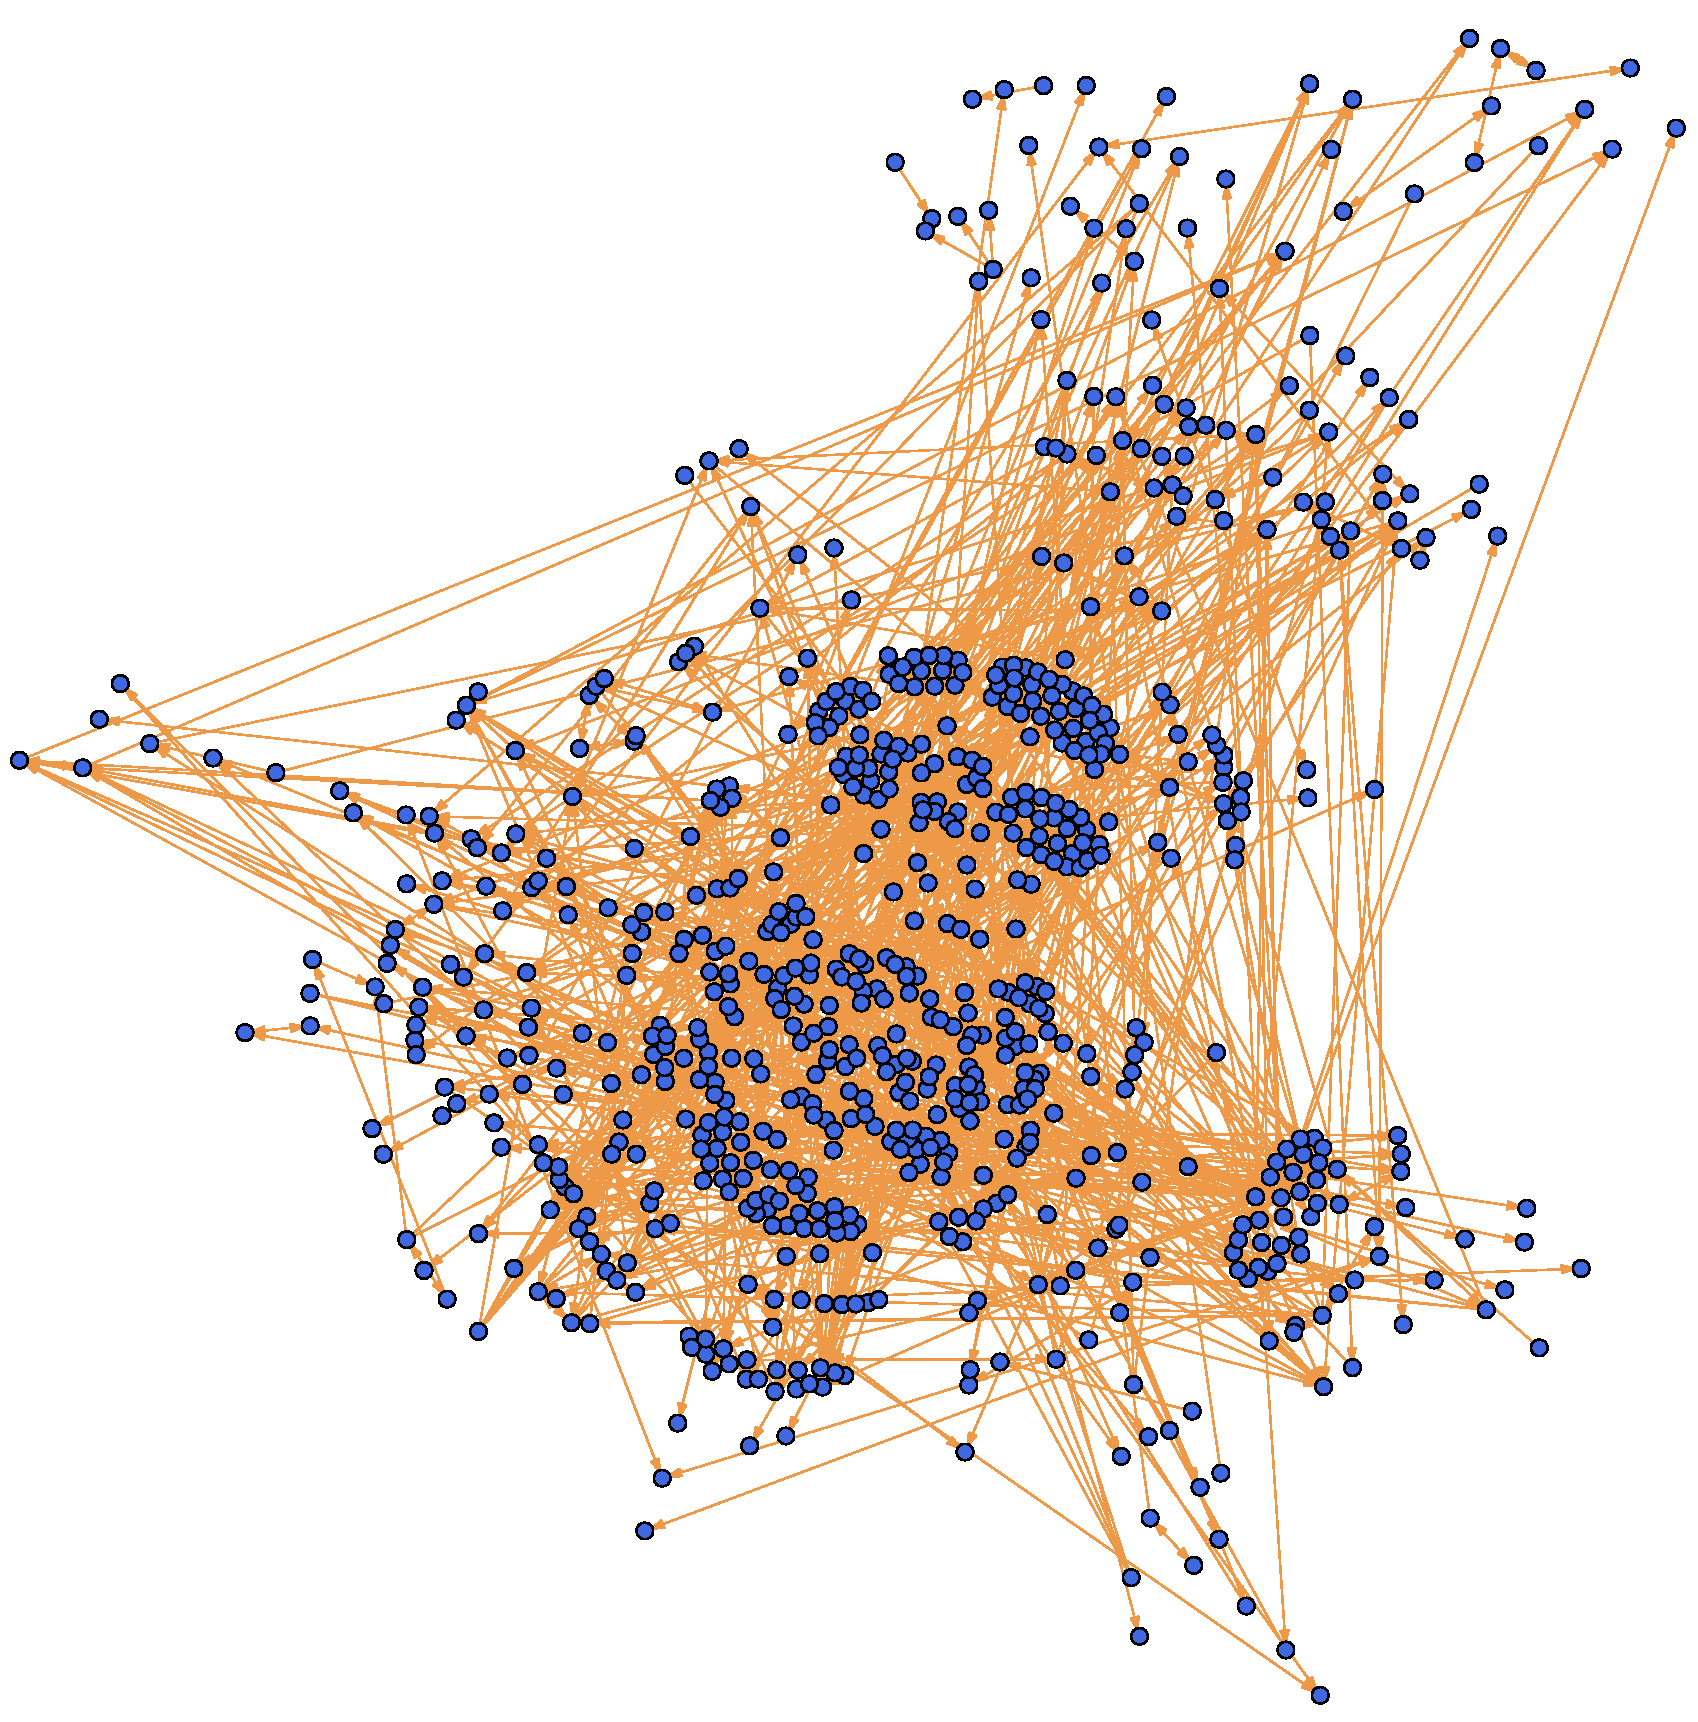
\includegraphics[width=0.8\linewidth]{GiantComp.pdf}
\captionof{figure}{Full graph of \textit{A. thaliana} L. protein-protein interaction network (layout Kamada-Kawai) }
\end{center}\vspace{.2cm}

Another small world model attribute of our PPI graph was the specified vertex degree distribution. Most common vertex degrees values laid between 1 and 10-11 (95\% of all vertices), only single nodes had degrees more than 20. Also, we could understand the manner in which vertices of different degrees are linked with each other nodes using of neighbors of a given vertex average degree. It suggests that although there is a tendency for vertices of higher degrees to link with similar nodes, also we have a small number of high-degree vertices linked with low-degree nodes. We can suppose that our PPI graph has 2 sets of high-degree vertices: ones that assert interaction transmission between big network compartments and other that connect within this parts. Vertices of lower degree tended to link with vertices of both lower and higher degrees. 

\begin{center}\vspace{.1cm}
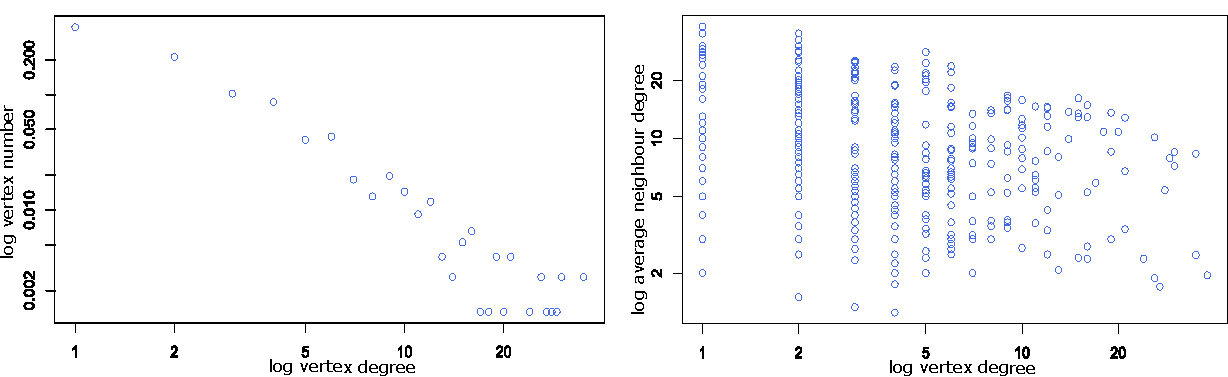
\includegraphics[width=1\linewidth]{degrees.pdf}
\captionof{figure}{Vertex degrees of \textit{A. thaliana} L. PPI graph}
\end{center}\vspace{.1cm}

\section*{Vertex and edge characteristics}

For the determination of protein "importance" in our network we used specialized algorithms including PageRank, HITS etc.  HITS algorithm generated two sets of vertices: authority (according to indegree level) and hubs (according to outdegree level. PageRank showed node "importance" using power method for computing the rank of nodes based on its backlink.  All algorithms showed sufficiently close results, therefore we could mark out some key proteins.

\begin{center}\vspace{.1cm}
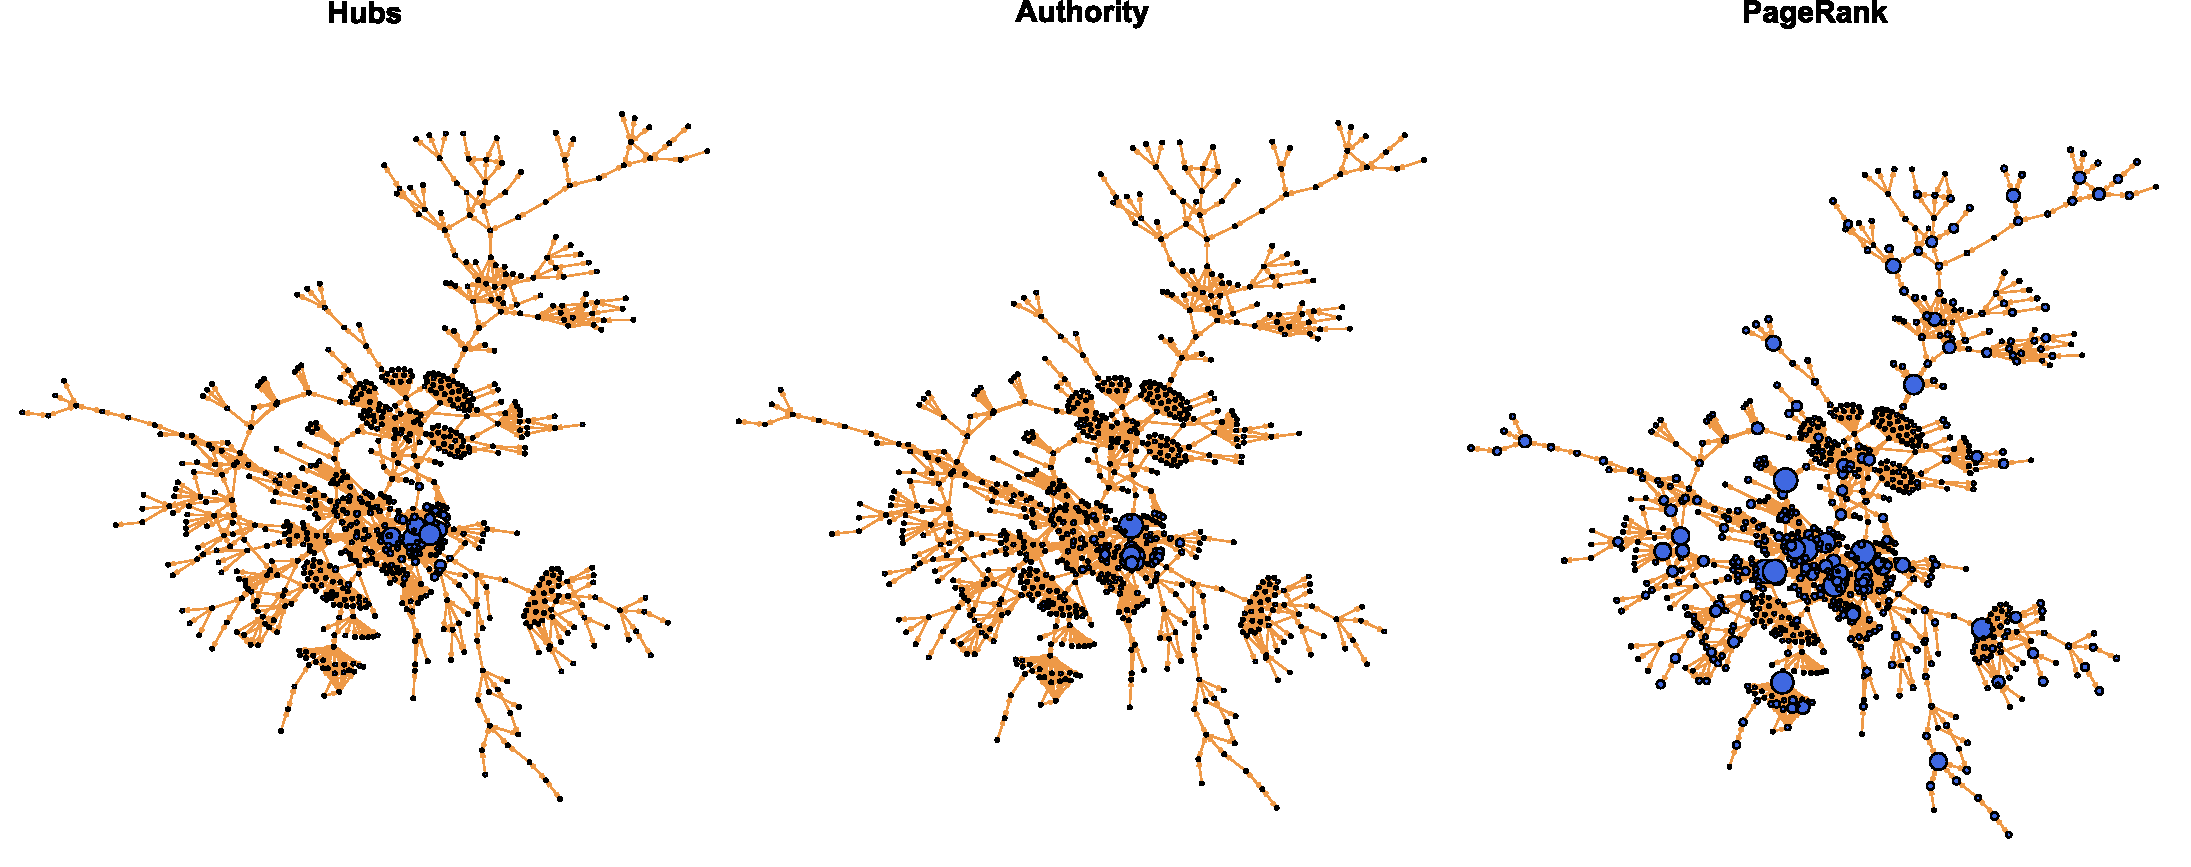
\includegraphics[width=1\linewidth]{vscores.pdf}
\captionof{figure}{Protein importance in \textit{A. thaliana} L. PPI network according to different algorithms}
\end{center}\vspace{.1cm}

In our PPI graph, 2-degree cliques were most prevalent, the maximal size of the cliques was six proteins. Four of six maximal clicks had 5 identical proteins (AT5G39760, AT4G24660, AT1G14440, AT1G75240, AT5G15210). Using K-cores algorithm we showed cores with degrees from one to eight (from 314 to 9 vertices). Another critical nodes was articulation points, that connected different parts of network.

For discovering the key links between proteins we used edge betweenness centrality (the number of shortest paths traversing that edge). It showed the links between nodes, that plays a key role in facilitating the direct flow of information inside network ($AT1G56280 \leftrightarrow AT1G35670$, $AT5G20570 \leftrightarrow AT5G46210$, $AT5G46210 \leftrightarrow AT4G05420$ and others). 


\begin{center}\vspace{1cm}
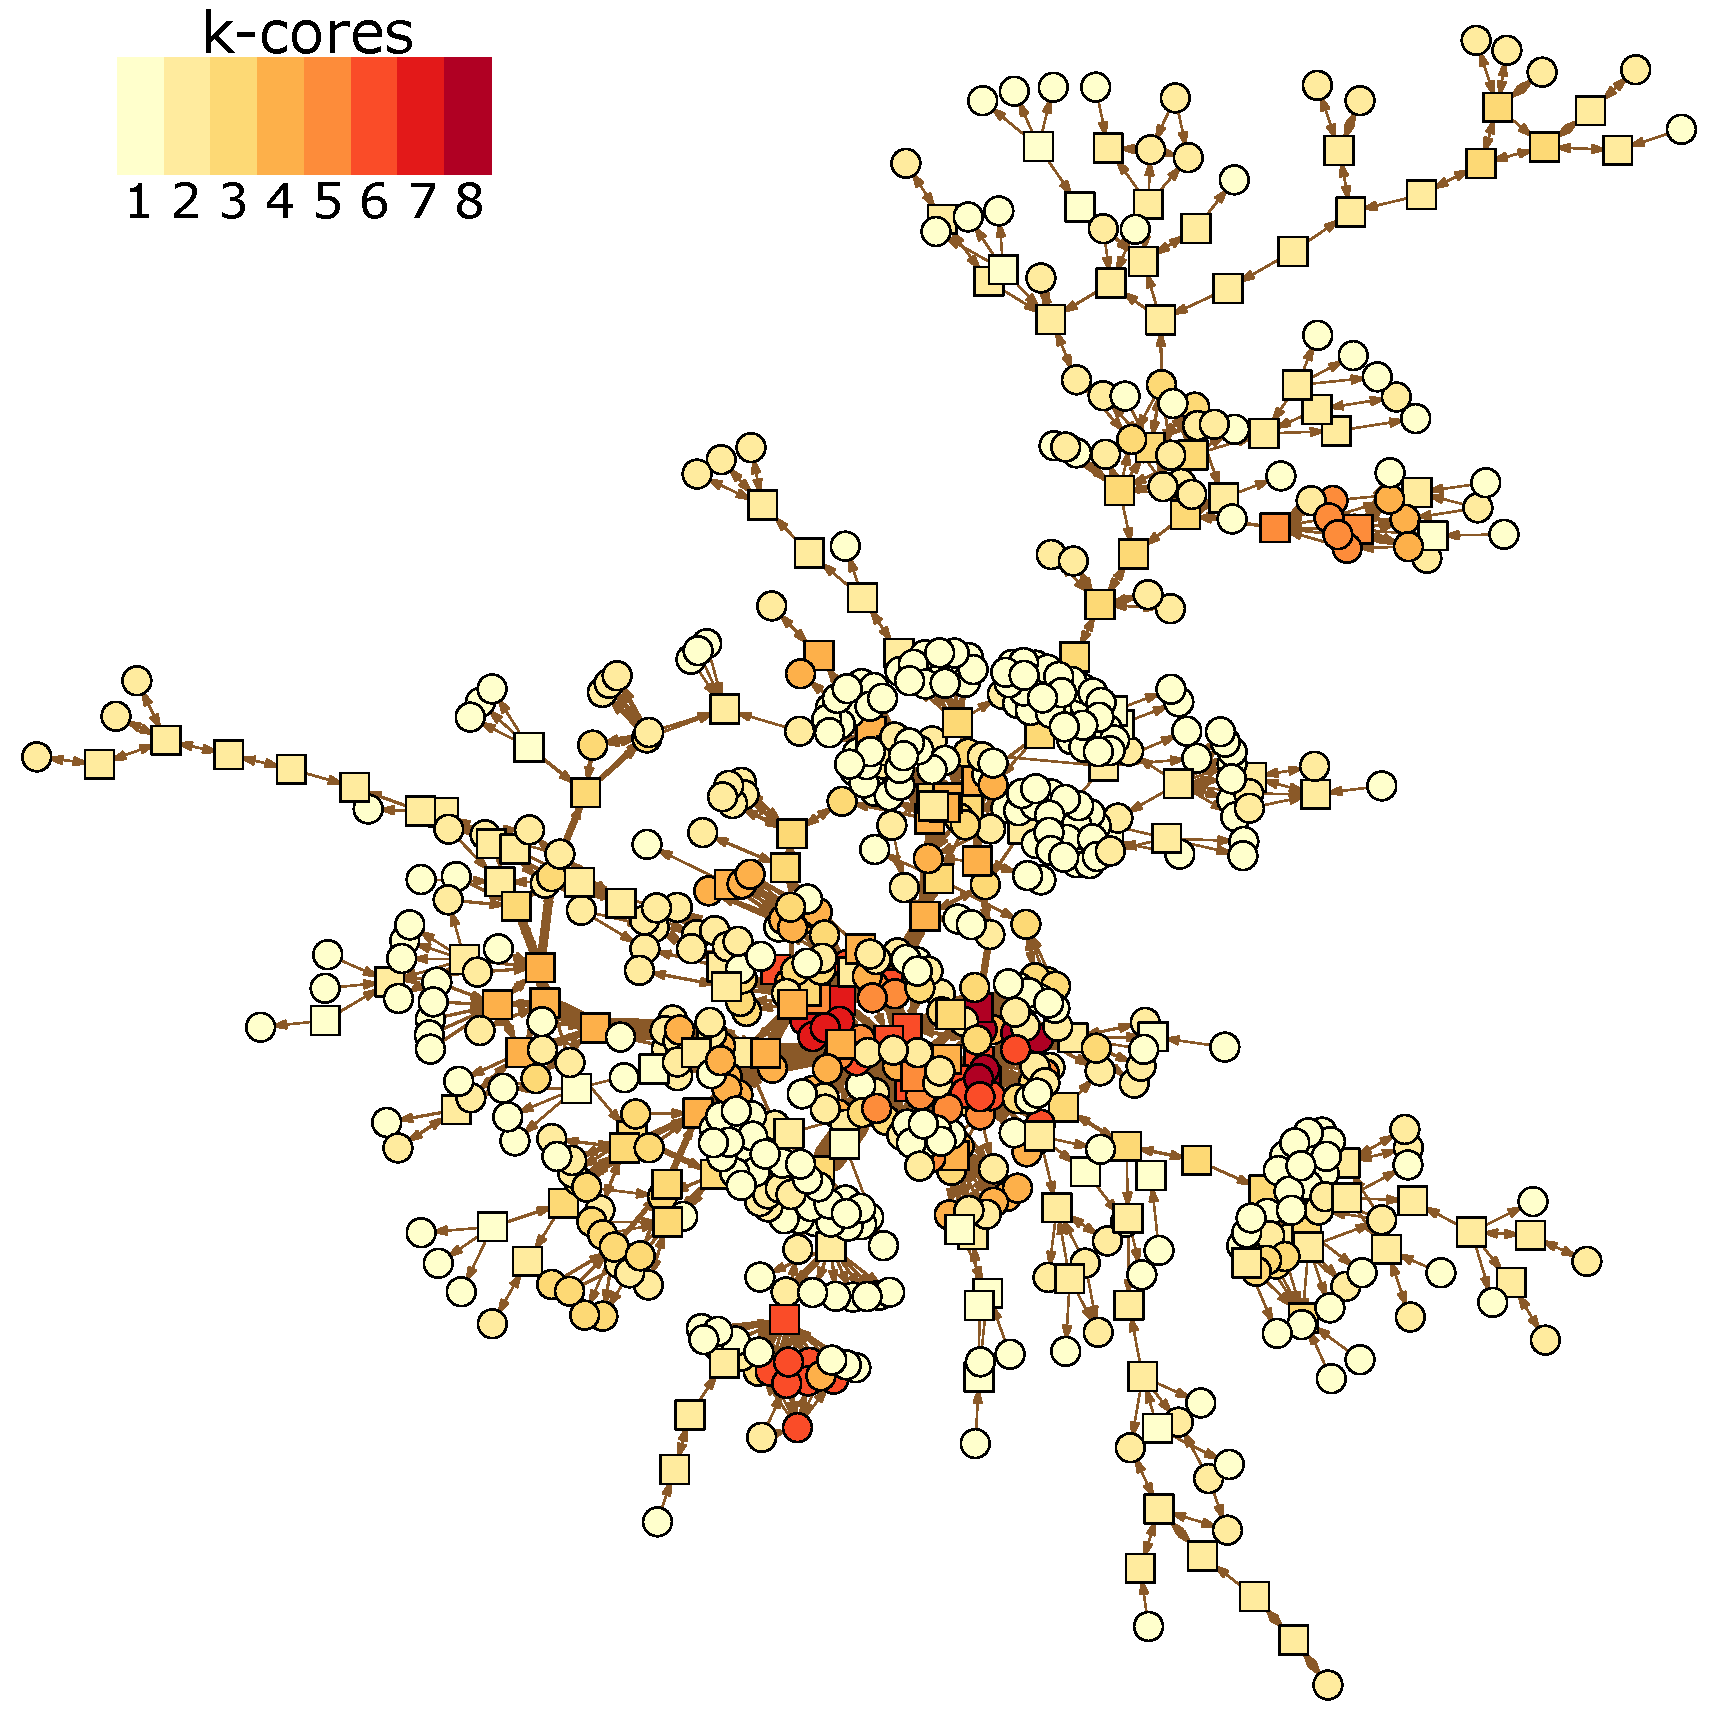
\includegraphics[width=0.8\linewidth]{cores.pdf}
\captionof{figure}{K-cores, articulation points ($\Box$) and edge betweenness centrality (lines width) in \textit{A. thaliana} L. PPI network }
\end{center}\vspace{1cm}


%----------------------------------------------------------------------------------------
%	CONCLUSIONS
%----------------------------------------------------------------------------------------

\color{SaddleBrown} % SaddleBrown color for the conclusions to make them stand out

\section*{Conclusions}

\begin{itemize}
\item We analyzed \textit{Arabidopsis thaliana} L. protein-protein interaction network using graph conception and specialized algorithms implemented in R programming language.
\item A full network is a graph consists of many subgraphs, including the fully-connected giant component with 763 vertices and 1393 edges, which was analyzed further. 
\item Our fully-connected graph has small world property and 2 sets of high-degree vertices: one that connects big network compartments and other that link with small-degree nodes within this parts.
\item Using different algorithms and (HITS, PageRank and others) we determined "important" proteins and connection between them.
\end{itemize}

\color{DarkSlateGray} % Set the color back to DarkSlateGray for the rest of the content

%----------------------------------------------------------------------------------------
%	FORTHCOMING RESEARCH
%----------------------------------------------------------------------------------------

\section*{Forthcoming Research}
Forthcoming investigations will include an extension of our graph using protein GO and interaction properties. This will allow us to research the correlation between proteins positions in the graph and theirs attributes for further network modeling. 

%	ACKNOWLEDGEMENTS
%----------------------------------------------------------------------------------------

\section*{Acknowledgements}

This research was supported by the grant of the Ministry of Education and Science of the Russian Federation (No 2016-220-05-163).

%----------------------------------------------------------------------------------------

\end{multicols}
\end{document}